\documentclass{beamer}

\mode<presentation> {

% The Beamer class comes with several default slide themes
% which change the colors and layouts of slides. Below this is a list
% of all the themes, uncomment each in turn to see what they look like.

%\usetheme{default}
\usetheme{AnnArbor}
%\usetheme{Antibes}
%\usetheme{Bergen}
%\usetheme{Berkeley}
%\usetheme{Berlin}
%\usetheme{Boadilla}
%\usetheme{CambridgeUS}
%\usetheme{Copenhagen}
%\usetheme{Darmstadt}
%\usetheme{Dresden}
%\usetheme{Frankfurt}
%\usetheme{Goettingen}
%\usetheme{Hannover}
%\usetheme{Ilmenau}
%\usetheme{JuanLesPins}
%\usetheme{Luebeck}
% \usetheme{Madrid}
% \usetheme{Malmoe}
%\usetheme{Marburg}
%\usetheme{Montpellier}
%\usetheme{PaloAlto}
% \usetheme{Pittsburgh}
%\usetheme{Rochester}
%\usetheme{Singapore}
%\usetheme{Szeged}
%\usetheme{Warsaw}

% As well as themes, the Beamer class has a number of color themes
% for any slide theme. Uncomment each of these in turn to see how it
% changes the colors of your current slide theme.

% \usecolortheme{albatross}
%\usecolortheme{beaver}
%\usecolortheme{beetle}
%\usecolortheme{crane}
% \usecolortheme{dolphin}
%\usecolortheme{dove}
%\usecolortheme{fly}
%\usecolortheme{lily}
%\usecolortheme{orchid}
% \usecolortheme{rose}
% \usecolortheme{seagull}
%\usecolortheme{seahorse}
%\usecolortheme{whale}
%\usecolortheme{wolverine}

%\setbeamertemplate{footline} % To remove the footer line in all slides uncomment this line
%\setbeamertemplate{footline}[page number] % To replace the footer line in all slides with a simple slide count uncomment this line

%\setbeamertemplate{navigation symbols}{} % To remove the navigation symbols from the bottom of all slides uncomment this line
}


\usepackage{graphicx} % Allows including images
\usepackage{caption}
\usepackage{booktabs} % Allows the use of \toprule, \midrule and \bottomrule in tables
\usepackage{tikz}
\usepackage{amsmath}
\usepackage{pgfplots}
\usepackage{hyperref}


\usetikzlibrary{arrows.meta, calc}

%----------------------------------------------------------------------------------------
%	TITLE PAGE
%----------------------------------------------------------------------------------------

\title[Calculus of Several Variables]{Geometric Interpretation of Derivatives in Higher Dimensions } % The short title appears at the bottom of every slide, the full title is only on the title page

\author{Hrisav Sarkar, BSC Mathematics} % Your name
\institute[Amity] % Your institution as it will appear on the bottom of every slide, may be shorthand to save space
{
Department of Mathematics, Amity University, Kolkata, India \\ % Your institution for the title page
\medskip
\textit{hrisav.sarkar@s.amity.edu } % Your email address
}
\date{6 February,2025} % Date, can be changed to a custom date


\begin{document}

\begin{frame}
\titlepage % Print the title page as the first slide
\end{frame}

\begin{frame}
\frametitle{Overview} % Table of contents slide, comment this block out to remove it
\tableofcontents % Throughout your presentation, if you choose to use \section{} and \subsection{} commands, these will automatically be printed on this slide as an overview of your presentation
\end{frame}

%----------------------------------------------------------------------------------------
%	PRESENTATION SLIDES
%----------------------------------------------------------------------------------------

%------------------------------------------------
\section{Introduction} % Sections can be created in order to organize your presentation into discrete blocks, all sections and subsections are automatically printed in the table of contents as an overview of the talk
%------------------------------------------------

\subsection{} % A subsection can be created just before a set of slides with a common theme to further break down your presentation into chunks

\begin{frame}
\frametitle{Introduction}
\begin{itemize}
    \item \textbf{Overview:}
      \begin{itemize}
        \item Extends the concept of derivatives from one-dimensional calculus to functions of several variables.
        \item Provides a framework for understanding how functions change along multiple directions.
      \end{itemize}
    \item \textbf{Key Ideas:}
      \begin{itemize}
        \item \textbf{Linear Approximation:} The derivative at a point is the best linear approximation of the function near that point.
      \end{itemize}
    \item \textbf{Why It Matters:}
      \begin{itemize}
        \item \textbf{Visualization:} Offers intuitive geometric insights into the behavior of multivariable functions.
        \item \textbf{Applications:} Fundamental in optimization, solving differential equations and modeling real-world phenomena.
      \end{itemize}
  \end{itemize}

\end{frame}
%------------------------------------------------
\section{Geometric Meaning of Derivative of a Vector Function } % Sections can be created in order to organize your presentation into discrete blocks, all sections and subsections are automatically printed in the table of contents as an overview of the talk
%------------------------------------------------
\subsection{} % A subsection can be created just before a set of slides with a common theme to further break down your presentation into chunks

\begin{frame}[allowframebreaks]
\frametitle{Geometric Meaning of the derivative of a vector Function}

The geometric meaning of the derivative of a vector function is closely related to the concept of the rate of change and the tangent vector.
\begin{itemize}
\item \textcolor{blue}{\textit{Rate of change of position}}:

\begin{block}{}
    Let $r:\mathbb{R}\rightarrow \mathbb{R}^n$, where $r$ is differentiable meaning $r(t)=(r_1(t),r_2(2),\cdots ,r_n(t))$ and all $r_i(t)$ such that $r_i:\mathbb{R}\rightarrow \mathbb{R}$ are differentiable functions, and $r'(t)=(r_1'(t),r_2'(2),\cdots ,r_n'(t))$ describes how the position of the vector-valued function $r(t)$ changes with respect to the parameter $t$.
\end{block}

\item \textcolor{blue}{\textit{Tangent Vector}}: 

\begin{block}{}
    $r'(t)$ at a specific point on the curve indicates the direction of the tangent line to the curve at that point.
\end{block}

\item \textcolor{blue}{\textit{Visualisation in 3D and 2D Spaces}}: \\
\begin{block}{}
    If a particle moving along a curve, $r'(t)$ at any point shows how the particle would continue moving if it maintains its current velocity and direction
\end{block}

\end{itemize} 
Consider the unit circle defined by 
  \[
  r(t) = (\cos t, \sin t).
  \]
  Its derivative is 
  \[
  r'(t) = (-\sin t, \cos t),
  \]
  Which represents the tangent vector at each point.

  At \(t=\frac{\pi}{4}\):
  \[
  r\Bigl(\frac{\pi}{4}\Bigr)=\Bigl(\frac{\sqrt{2}}{2}, \frac{\sqrt{2}}{2}\Bigr),
  \]
  \[
  r'\Bigl(\frac{\pi}{4}\Bigr)=\Bigl(-\frac{\sqrt{2}}{2}, \frac{\sqrt{2}}{2}\Bigr).
  \]
  
  The tangent line is then given by
  \[
  L(s)=r\Bigl(\frac{\pi}{4}\Bigr) + s\,r'\Bigl(\frac{\pi}{4}\Bigr)
  = \Bigl(\frac{\sqrt{2}}{2}, \frac{\sqrt{2}}{2}\Bigr) + s\Bigl(-\frac{\sqrt{2}}{2}, \frac{\sqrt{2}}{2}\Bigr),
  \quad s\in\mathbb{R}.
  \]
\begin{center}
    
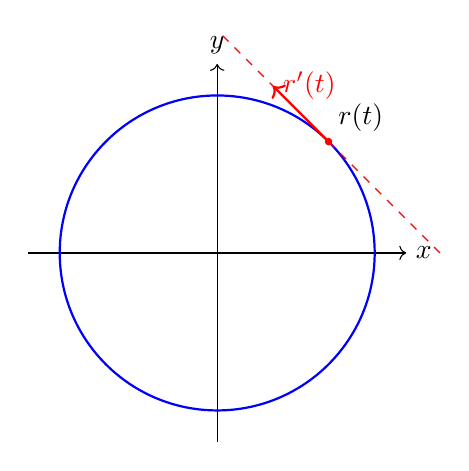
\begin{tikzpicture}[scale=2]
  % Draw coordinate axes
  \draw[->] (-1.2,0) -- (1.2,0) node[right] {$x$};
  \draw[->] (0,-1.2) -- (0,1.2) node[above] {$y$};
  
  % Draw the unit circle (our curve)
  \draw[thick,blue] (0,0) circle (1);
  
  % Define the point of tangency for t = 45° (π/4)
  \def\angle{45}
  \coordinate (P) at ({cos(\angle)}, {sin(\angle)});
  
  % Mark the point on the curve
  \filldraw[red] (P) circle (0.02);
  \node[above right] at (P) {$r(t)$};
  
  % For the unit circle, r'(t) = (-sin t, cos t).
  % At t=45° this is (-sin 45°, cos 45°).
  \pgfmathsetmacro{\dx}{-sin(\angle)}
  \pgfmathsetmacro{\dy}{cos(\angle)}
  
  % Draw the tangent vector at P (scaled down for clarity)
  \draw[->,red,thick] (P) -- ++({\dx/2},{\dy/2}) node[right] {$r'(t)$};
  
  % Draw the full tangent line through P.
  % Parametric form: (x,y) = (cos 45, sin 45) + s * (-sin 45, cos 45).
  \draw[dashed,red] plot[domain=-1:1] 
    ({cos(\angle) + \dx*\x},{sin(\angle) + \dy*\x});
\end{tikzpicture}
\end{center}
\captionof{figure}{A unit circle with its tangent vector and the tangent line at $t=\pi/4$.}
\end{frame}

\section{Significance of Gradient}

\subsection{Understanding the Gradient of a Function}

\begin{frame}{Understanding the Gradient of a Function}

    \textbf{What is the Gradient?} \\
    The \textbf{gradient} of a function is a vector that tells us two things:
    \begin{itemize}
        \item \textbf{Direction} – Where the function increases the fastest.
        \item \textbf{Steepness} – How fast the function increases in that direction.
    \end{itemize}

    Mathematically, for a function \( f(x, y) \), the gradient is written as:
    \[
    \nabla f = \left( \frac{\partial f}{\partial x}, \frac{\partial f}{\partial y} \right)
    \]
    This means:
    \begin{itemize}
        \item \( \frac{\partial f}{\partial x} \) tells how much \( f \) changes as we move in the \( x \)-direction.
        \item \( \frac{\partial f}{\partial y} \) tells how much \( f \) changes as we move in the \( y \)-direction.
    \end{itemize}

\end{frame}

\subsection{Example: Climbing a Hill}

\begin{frame}{Example: Climbing a Hill}
    Imagine you are hiking on a hill where the height at any point is given by \( f(x, y) \).
    \begin{itemize}
        \item The \textbf{gradient} tells you the steepest path to climb up.
        \item The bigger the gradient’s length, the steeper the climb.
    \end{itemize}

    \textbf{Mathematical Example:} If \( f(x, y) = x^2 + y^2 \), then:
    \[
    \nabla f = (2x, 2y)
    \]
    \begin{itemize}
        \item At \( (1,1) \), the gradient is \( (2,2) \), meaning the function increases fastest in the \((1,1)\) direction.
        \item At \( (0,0) \), the gradient is \( (0,0) \), meaning it’s a flat point (no steepest direction).
    \end{itemize}
    
    \centering
    % \includegraphics[width=0.5\linewidth]{gradienthill.png} % Add a relevant figure here

\end{frame}

\subsection{Geometric Meaning}

\begin{frame}{Geometric Meaning}
    \begin{itemize}
        \item The \textbf{gradient vector} always points in the direction where the function increases the fastest.
        \item The \textbf{steepness} (magnitude of the gradient) tells how quickly the function increases.
        \item The gradient is \textbf{perpendicular} to the level curves (contour lines).
    \end{itemize}
\end{frame}

\subsection{Physical Meaning (Real-World Examples)}
\begin{frame}{Physical Meaning (Real-World Examples)}
    The gradient is useful in many areas of science:
    \begin{itemize}
        \item \textbf{Heat Flow:} If \( f(x, y) \) represents temperature, then \( \nabla f \) shows the direction where heat increases fastest.
        \item \textbf{Electric Fields:} The gradient of voltage tells us how electric potential changes in space.
        \item \textbf{Water Flow:} Water flows \textbf{downhill}, opposite to the gradient of elevation.
    \end{itemize}
    
    \centering
    % \includegraphics[width=0.5\linewidth]{gradient_real_world.png} % Add a relevant figure here

\end{frame}

\begin{frame}[allowframebreaks]{Gradient of a Scalar-Valued Function Figure}

    \begin{figure}[h]
    \centering
    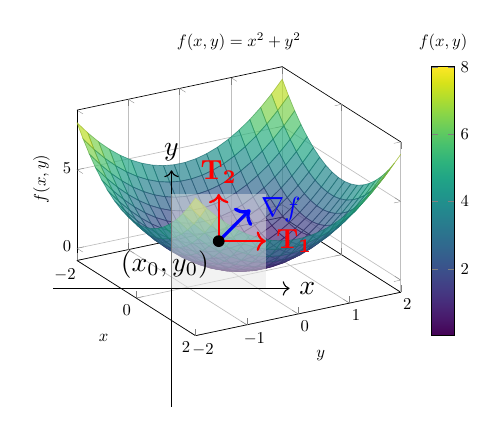
\begin{tikzpicture}[scale=0.6]
        % Define the function f(x, y) = x^2 + y^2
        \begin{axis}[
            view={60}{30},
            xlabel={$x$},
            ylabel={$y$},
            zlabel={$f(x,y)$},
            domain=-2:2,
            y domain=-2:2,
            samples=20,
            grid=major,
            colormap/viridis,
            colorbar,
            colorbar style={title={$f(x,y)$}},
            title={$f(x,y) = x^2 + y^2$}
        ]
            \addplot3[
                surf,
                opacity=0.7
            ] {x^2 + y^2};
        \end{axis}

        % Define the chosen point (x0, y0)
        \def\xo{1}
        \def\yo{1}
        \def\fo{1^2 + 1^2} % Function value at (x0, y0)
        \def\gradx{2 * \xo}  % Partial derivative df/dx at (x0, y0)
        \def\grady{2 * \yo}  % Partial derivative df/dy at (x0, y0)

        % Shifted 3D tangent plane representation
        \begin{scope}[shift={(2,1)}]
            % Axes in xy-plane
            \draw[->] (-2.5, 0) -- (2.5, 0) node[right] {$x$};
            \draw[->] (0, -2.5) -- (0, 2.5) node[above] {$y$};

            % Draw tangent plane at (x0, y0)
            \fill[gray!20, opacity=0.5] 
                (\xo-1, \yo-1) -- (\xo+1, \yo-1) -- 
                (\xo+1, \yo+1) -- (\xo-1, \yo+1) -- cycle;

            % Gradient vector perpendicular to tangent plane
            \draw[->, blue, very thick] (\xo, \yo) -- ++(\gradx/3, \grady/3) node[right] {$\nabla f$};

            % Tangent plane direction vectors
            \draw[->, red, thick] (\xo, \yo) -- ++(1, 0) node[right] {$\mathbf{T_1}$};
            \draw[->, red, thick] (\xo, \yo) -- ++(0, 1) node[above] {$\mathbf{T_2}$};

            % Mark point on xy-plane
            \node[fill=black, circle, inner sep=1.5pt] at (\xo, \yo) {};
            \node[below left] at (\xo, \yo) {$(x_0, y_0)$};
        \end{scope}

    \end{tikzpicture}
    \caption{Illustration of the function \( f(x,y) = x^2 + y^2 \), its tangent plane at \( (1,1) \), and the gradient vector perpendicular to the plane.}
\end{figure}

\end{frame}


% \begin{frame}[fragile] % Need to use the fragile option when verbatim is used in the slide
% \frametitle{Citation}
% An example of the \verb|\cite| command to cite within the presentation:\\~

% This statement requires the citation \cite{p1}.
% \end{frame}

% %------------------------------------------------

% \begin{frame}
% \frametitle{References}
% \footnotesize{
% \begin{thebibliography}{99} % Beamer does not support BibTeX so references must be inserted manually as below
% \bibitem[Smith, 2012]{p1} John Smith (2012)
% \newblock Title of the publication
% \newblock \emph{Journal Name} 12(3), 45 -- 678.
% \end{thebibliography}
% }
% \end{frame}

% %------------------------------------------------

\begin{frame}
\Huge{\centerline{The End}}
\end{frame}

%----------------------------------------------------------------------------------------

\end{document}